\chapter{Conceito do negócio}

Existem três componentes cruciais para um novo negócio bem sucedido: a
oportunidade, o emprededor (e o time de gerenciamento, se é um negócio 
de alto risco) e os recursos necessários para iniciar a empresa e fazê-la
crescer \cite{bygrave2010entrepreneurship}. %página 56
Estes três componentes devem se encaixar bem.
A figura \ref{componentes} mostra como os componentes são relacionados.
No centro deste \textit{framework}
está o plano de negócio, o resultado da integração dos três ingredientes
básicos para um plano estratégico completo para o novo negócio.
Não é suficiente ter uma ideia de primeira para um novo negócio se você tem 
um time de gerenciamento de segunda.  Assim como ter apenas ideias e gerenciamento
não é bom sem os recursos apropriados. 

\begin{figure}[!h]
	\begin{center}
		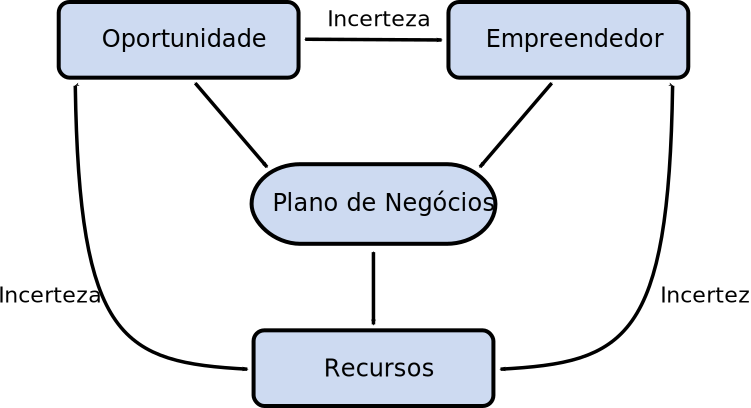
\includegraphics[scale=0.5]{../slides/imagens/componentes.pdf}
	\end{center}
	\caption{\label{componentes} O relacionamento dos três componentes, baseado no 
		\textit{framework} de Jeffry Timmons \cite{timmons2004new}.}			
\end{figure}

A força motriz crucial para qualquer tipo de tomada de risco é o empreendedor
líder e o grupo de gerenciamento fundador.

\section{A oportunidade}

O maior equívoco sobre a ideia para um novo negócio é que ela deve ser
única.  A função de um empreendedor implica na descoberta, avaliação
e exploração de oportunidades, em outras palavras, de novos produtos, 
serviços ou processos de produção; novas estratégias e formas
organizacionais para novos mercados para produtos
e entradas que anteriormente não existiam \cite{fayolle2007handbook}.
A oportunidade de um empreendedor é uma ideia que ainda não foi 
avaliada economicamente ou não era esperada \cite{cuervo2007entrepreneurship}.

A ideia em si não é o mais importante.  No empreendedorismo, o 
desenvolvimento da ideia, a implementação e a construção de negócios bem
sucedidos é o que realmente importa.  Quando Alexander Fleming descobriu
a penicilina por acaso, nunca pensou em desenvolvê-la como uma droga.
Somente dez anos depois que Ernst Chain e Howard Florey viram o
seu potencial uso, e logo ela estava sendo utilizada para tratar pacientes
na Inglaterra.
